%!TEX root = ../template.tex
%%%%%%%%%%%%%%%%%%%%%%%%%%%%%%%%%%%%%%%%%%%%%%%%%%%%%%%%%%%%%%%%%%%%
%% chapter5.tex
%% NOVA thesis document file
%%
%% Chapter with the robotic system description.
%%%%%%%%%%%%%%%%%%%%%%%%%%%%%%%%%%%%%%%%%%%%%%%%%%%%%%%%%%%%%%%%%%%%
\chapter{Robotic System}
\label{cha:robotic_system}

\begin{quotation}
\begin{flushright}
\itshape
«It's a lot like nuts and bolts - if the rider's nuts, the horse bolts!»\\
\textbf{- Nicholas Evans}
\end{flushright}
\end{quotation}

This chapter's goal is to describe in detail the robotic system used on this thesis. It will start with a general overview of the robot. It follows with a physical description of all the parts, safety considerations and installation procedure. The way to operate the robot and the operation limits will also be presented. The chapter will end with an overview of the integrations with \gls{ros} and Gazebo.

% ==========================
% = Overview =
% ==========================

\section{Overview}
\label{sec:robotic_system_overview}

The robotic system is a robotic manipulator arm called Panda, from the german company Franka Emika GmbH (Fig. \ref{fig:franka_panda_overview}). It is an award winning robot in the category of collaborative robotics. It first won the Deutscher Zukunftspreis prize in 2017. On the following year, 2018, it also won the Time Best Inventions prize and German Innovation Award. In 2019, it won the iF Product Design Award \cite{FrankaEmikaGmbH_official_website}. 

\begin{figure}[htbp]
	\centering
	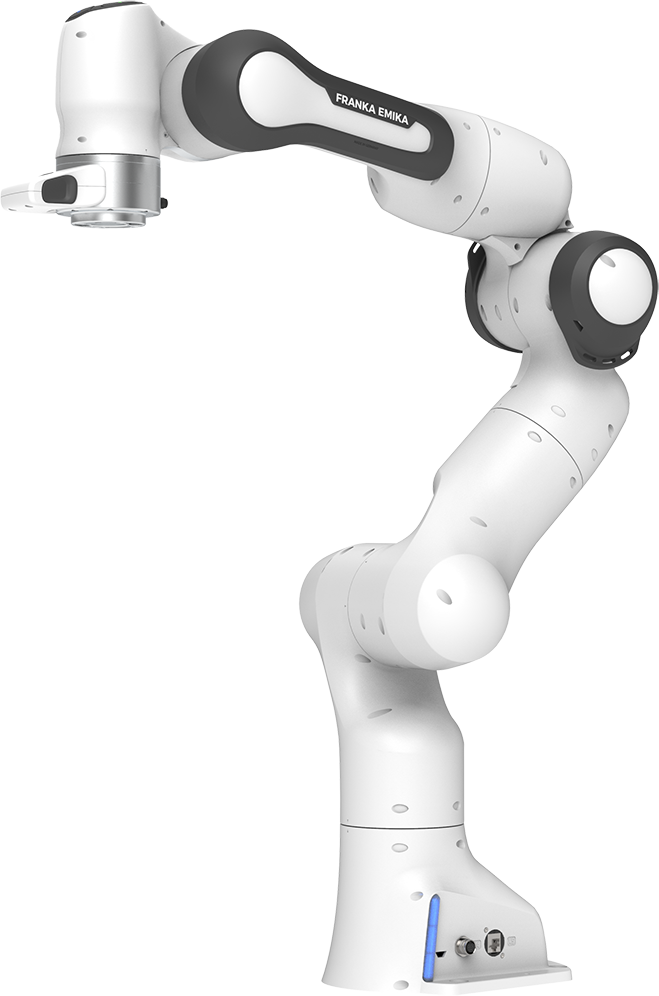
\includegraphics[width=.3\textwidth]{franka_panda_overview}
	\caption{Panda robotic manipulator arm from Franka Emika GmbH. Courtesy of Franka Emika GmbH, from the press kit available on \cite{FrankaEmikaGmbH_official_website}.}
	\label{fig:franka_panda_overview}
\end{figure}

The robot has seven degrees-of-freedom given from seven revolute joints. From a technology point-of-view, the joints are advanced mechatronic mechanisms. Each joint has a 14 bits resolution positional encoder. The motors used are a proprietary technology of brushless dc motors that are connected to strain wave gears for zero backlash. The joints also have torque sensors with 13 bits resolution. This complex joint system is controlled via real time electronics at 1 kHz rate \cite{FrankaEmikaGmbH_technology}.

The technology used on the joints contributes for the good operational results which robot has. Regarding free space motion the robot has a pose repeatabillity error of $\pm \SI{0.1}{\milli\meter}$ and a path deviation error of $\pm \SI{1.25}{\milli\meter}$. The torque sensors provide a resolution under 0.05 N on the forces measured at the end-effector. The force accuracy is 0.8 N and it has a repeatabillity under 0.05 N. The robot can apply forces to a minimum of 0.05 N at 1 kHz. Another characteristic of the robot is its collision detection capabilities. It can detect collisions in less than 2 ms, and react to it in less than 50 ms. More details are described on annex \ref{ann:panda_datasheet}.

The robot versatility allows it to be used on a broad range of tasks. In a factory setting, it can be used for parts assembly, pick-and-place, and physical manipulation of tools. In conjunction with vision systems it can be used for visual inspection, sorting, and other vision-based tasks. Outside of the factory, these skills can be used to automate other processes that require the same skills. Another important point is that being a collaborative robot, it can work safely side-by-side with a human.

Besides all the physical capabilities, on the software side, the system comes with a web-based interface called \emph{Desk} to program the robot via apps. This system simplifies the configuration of specific tasks for the robot to execute. The tasks can be saved and even distributed across various robots. For research purposes, the robot comes with a control interface, \gls{fci}, that allows the user to create custom made controllers. This is the interface used on this thesis.

% section robotic_system_overview

% ==========================
% = Physical Description =
% ==========================

\section{Physical Description}
\label{sec:robotic_system_physical_description}

The basic setup of the robot system is shown on Figure \ref{fig:robotic_system_basic_setup}. It shows the Panda \emph{Arm} with the \emph{Hand} end-effector. Along with it, there is the \emph{Control} hardware; the \emph{Host PC}, to connect to Desk and/or Control; and the security devices. Each one will be described in more detail.

\begin{figure}[htbp]
	\centering
	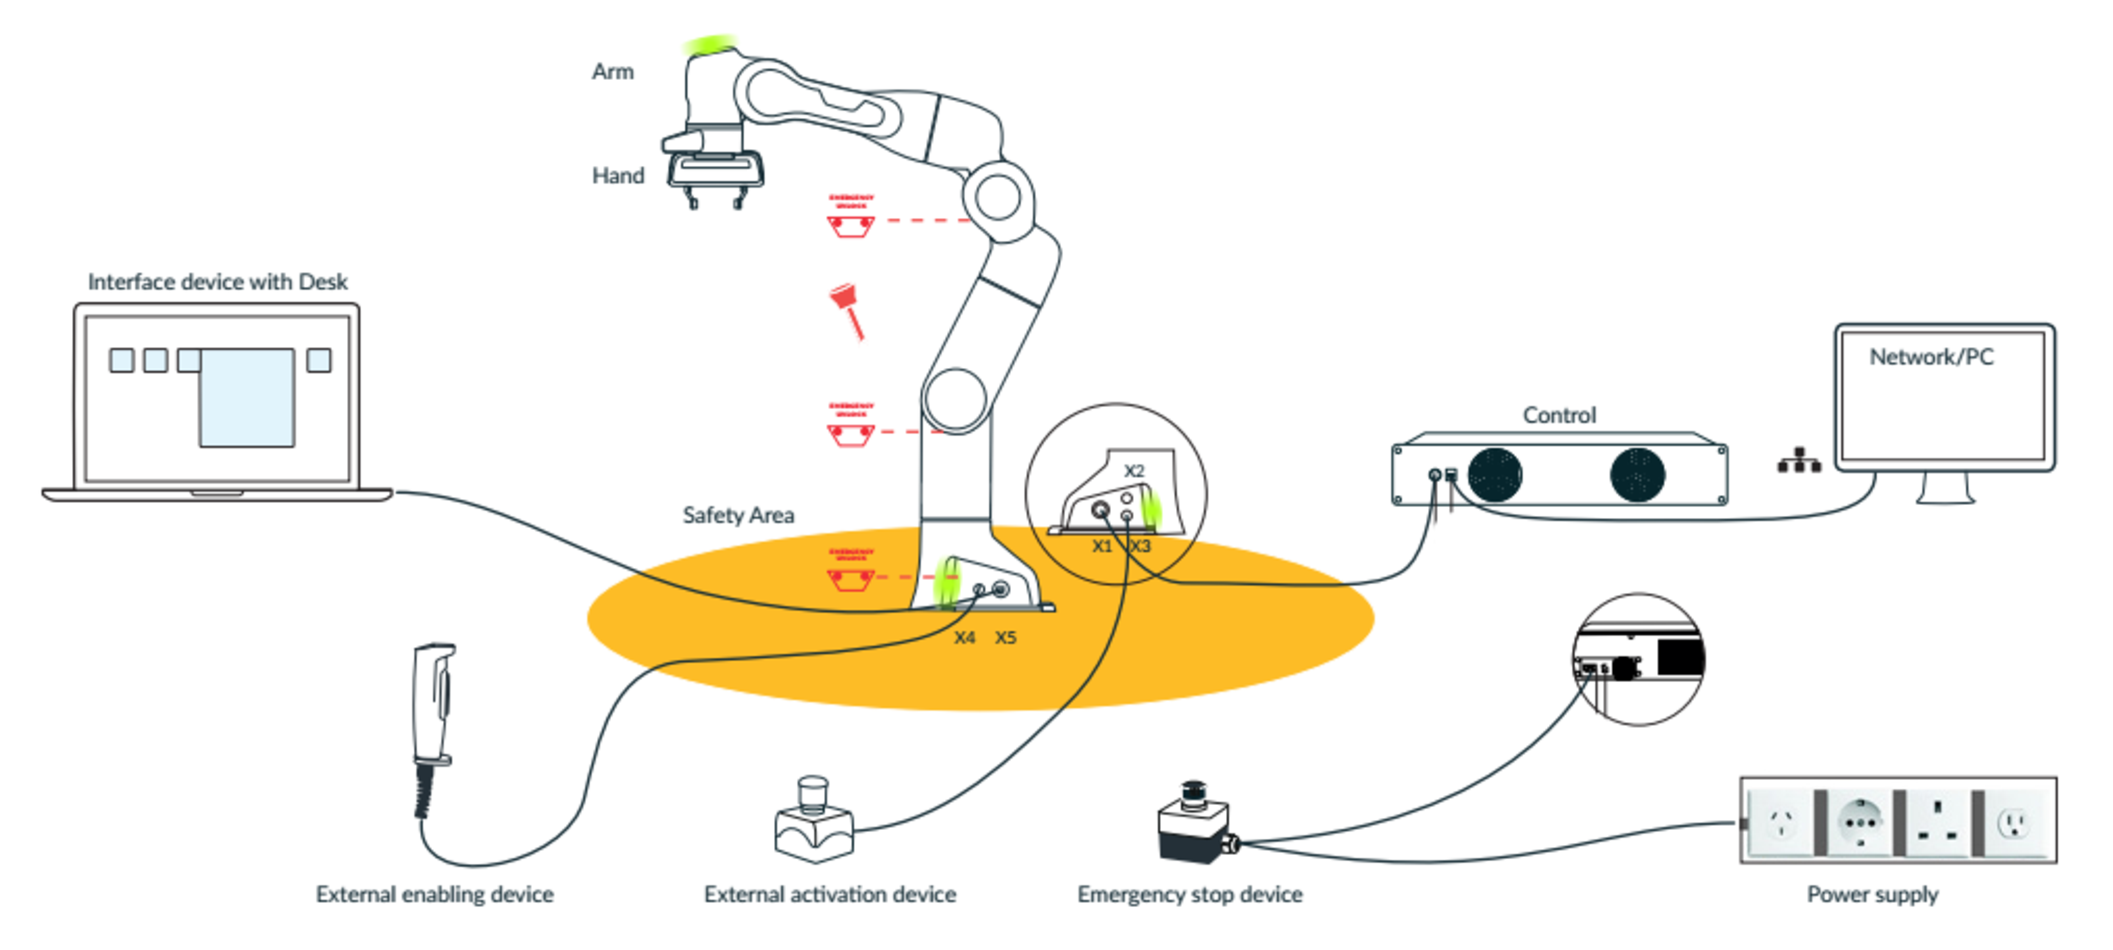
\includegraphics[width=\textwidth]{panda_basic_setup}
	\caption{Basic setup of the robotic system. Courtesy of Franka Emika GmbH and adapted from Panda user handbook of 2018.}
	\label{fig:robotic_system_basic_setup}
\end{figure}

\subsection*{Panda Arm}
\label{subsec:robotic_system_physical_description_panda_arm}

The Panda Arm is the main part of the robotic system. As previously mentioned, it has seven revolute joints, making it a redundant robot for any task in 3D space.

\begin{figure}[htbp]
	\centering
	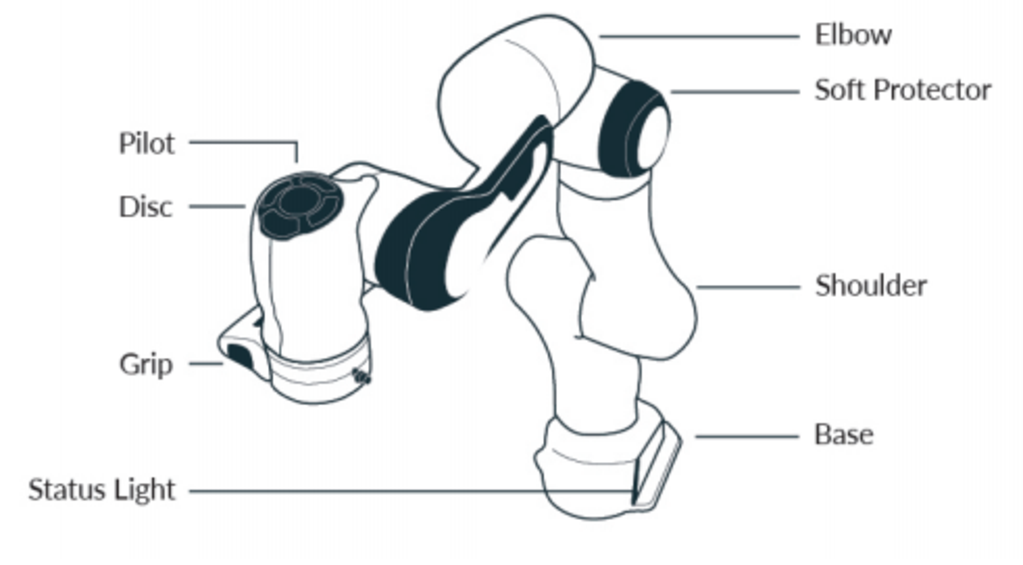
\includegraphics[width=0.8\textwidth]{panda_arm_components}
	\caption{Components of the Panda Arm. Courtesy of Franka Emika GmbH and adapted from Panda user handbook of 2018.}
	\label{fig:panda_arm_components}
\end{figure}

The Arm has several components worth mentioning (Fig. \ref{fig:panda_arm_components}). At the base of the robot there are two LED strip lights to indicate the status of the robot. These will be explained on section \ref{sec:robotic_system_operation}. Two of the joints have special names because of their resemblance to a human arm. The second joint is called \emph{Shoulder} and the fourth joint is called \emph{Elbow}. These are common joint names for anthropomorphic-like robot arms. The last link also has a special name, it is called \emph{Pilot}. It acts as a control platform for the robot. It works in conjunction with the Desk interface. The Pilot has the \emph{Disc} which is a set of control buttons, and the \emph{Grip}, which allows the user to manually guide the robot when in \emph{interactive} or "monitored stop" mode. The Pilot is show in more detail on Figure \ref{fig:panda_pilot_topview}.

\begin{figure}[htbp]
    \centering
	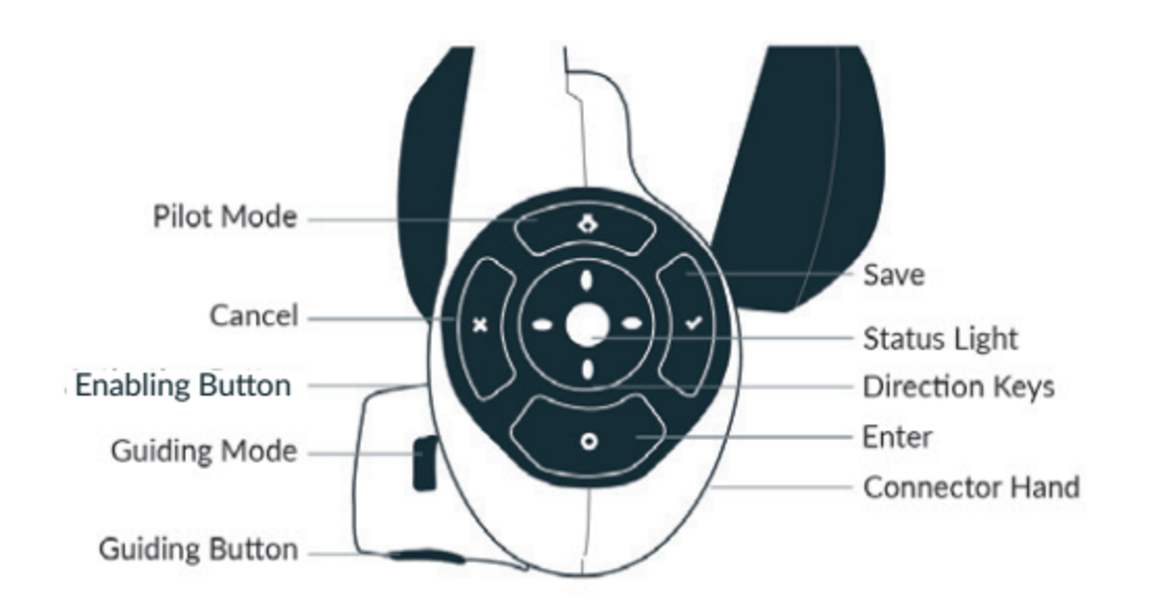
\includegraphics[width=0.8\textwidth]{panda_pilot_topview}
	\caption{Detailed view of Panda Arm Pilot. Courtesy of Franka Emika GmbH and adapted from Panda user handbook of 2018.}
	\label{fig:panda_pilot_topview}
\end{figure}

% subsection robotic_system_physical_description_panda_arm

\subsection*{Panda Hand}
\label{subsec:robotic_system_physical_description_panda_hand}

On a typical assembly of the Panda Arm, the end-effector used is the Panda Hand, which is the official end-effector. This tool is a two-finger, linear single axis robot hand (Fig. \ref{fig:panda_hand}). The Hand is powered directly from the Arm via a proprietary cable. The fingers can change positions in order to increase the span length. They can also be easily replaced by custom made fingers fitted for the task in hand. The fingertips can also be replaced in order to adapt the gripping format and strength to a specific task.

\begin{figure}[htbp]
    \centering
	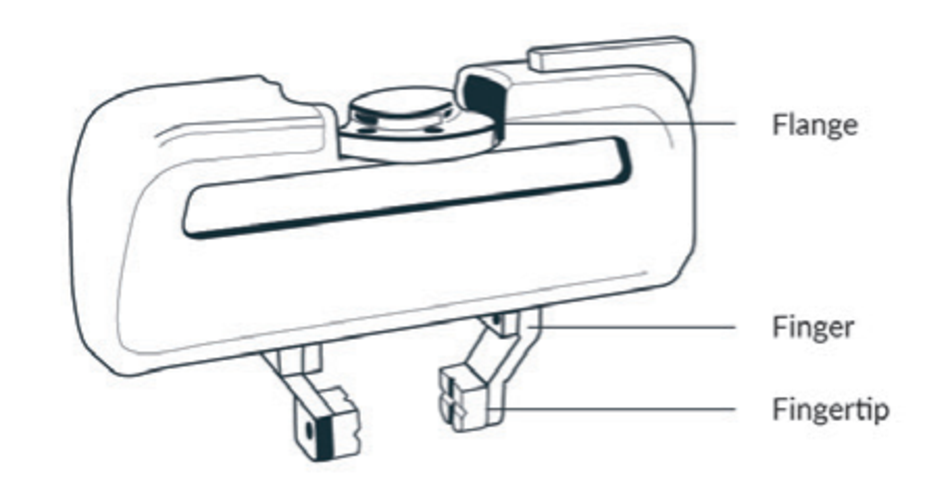
\includegraphics[width=0.8\textwidth]{panda_hand}
	\caption{Panda Hand. Courtesy of Franka Emika GmbH and adapted from Panda user handbook of 2018.}
	\label{fig:panda_hand}
\end{figure}

% subsection robotic_system_physical_description_panda_hand

\subsection*{Control}
\label{subsec:robotic_system_physical_description_control}

The Control is a special computer responsible for controlling the Panda Arm (Fig. \ref{fig:panda_control}). Without control the arm does not work. They are physically connected via a control cable. To control the robot via \gls{fci} the Host PC and the Control need to be connected via a RJ-45 ethernet cable. Otherwise, the Host PC can be directly connected to the Panda Arm base via the same cable.

\begin{figure}[htbp]
    \centering
	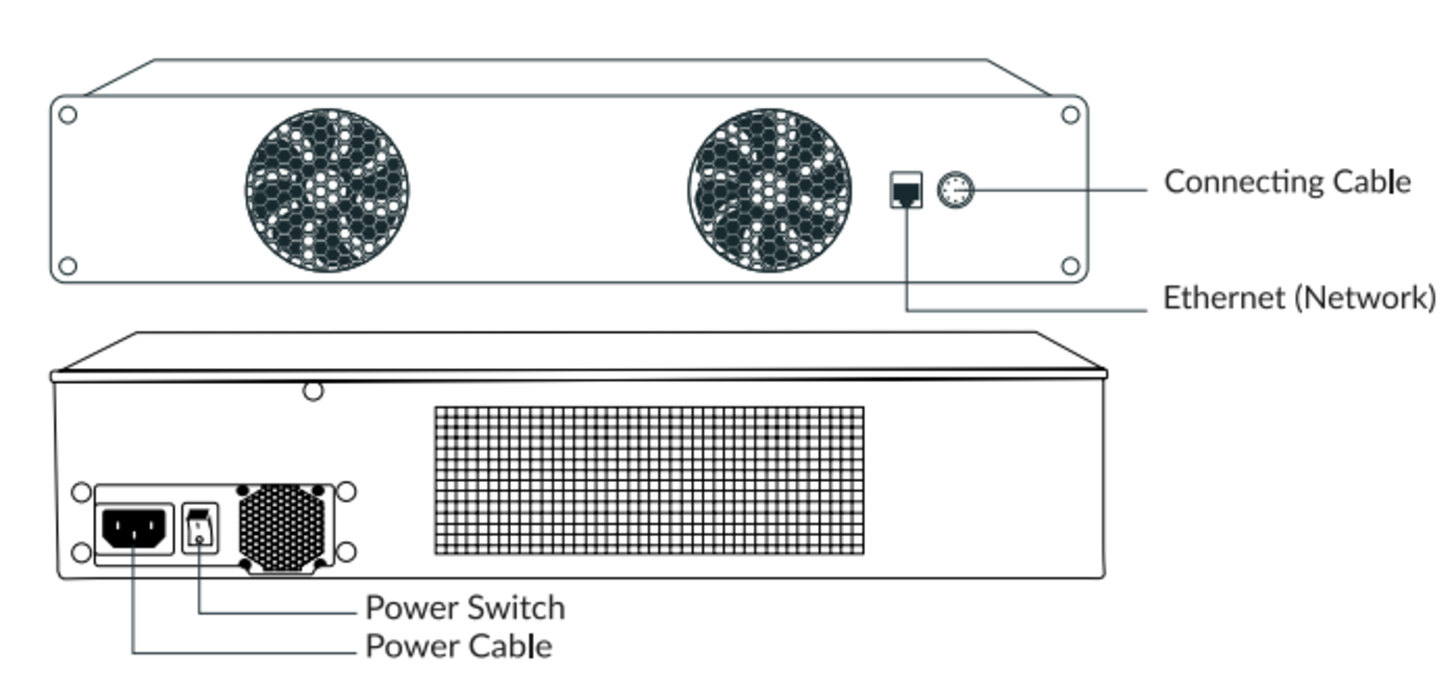
\includegraphics[width=0.8\textwidth]{panda_control}
	\caption{Panda Control hardware. Courtesy of Franka Emika GmbH and adapted from Panda user handbook of 2018.}
	\label{fig:panda_control}
\end{figure}

% subsection robotic_system_physical_description_control

\subsection*{Safety devices}
\label{subsec:robotic_system_physical_description_safety_devices}

The robot comes with three safety devices (Fig. \ref{fig:panda_safety_devices}) that allow the user to stop the robot immediately when needed. \\
The emergency stop device (Fig. \ref{fig:panda_safety_devices}c) is connected between the Control and mains power. The button has two states. When pressed down it is an open switch. When the button is lifted, the switch is closed and the Control is powered. \\
The external activation device (Fig. \ref{fig:panda_safety_devices}b) behaves similarly to the emergency stop device. When the button is pressed the robot is stopped and stays on the interactive mode. It can only be manually moved via the Grip buttons on the Pilot. When the button is lifted the robot goes to activated mode. In this mode the Desk tasks can be executed and the custom controllers can be run. If the button is pressed while the robot is moving it will stop immediately.
Finally, the external enabling device (Fig. \ref{fig:panda_safety_devices}a) is used to bypass the activation device. If the button is half pressed it goes to the activated mode and the Desk tasks can be run. If the button is not pressed or full pressed it will stop the robot.

\begin{figure}[htbp]
    \centering
	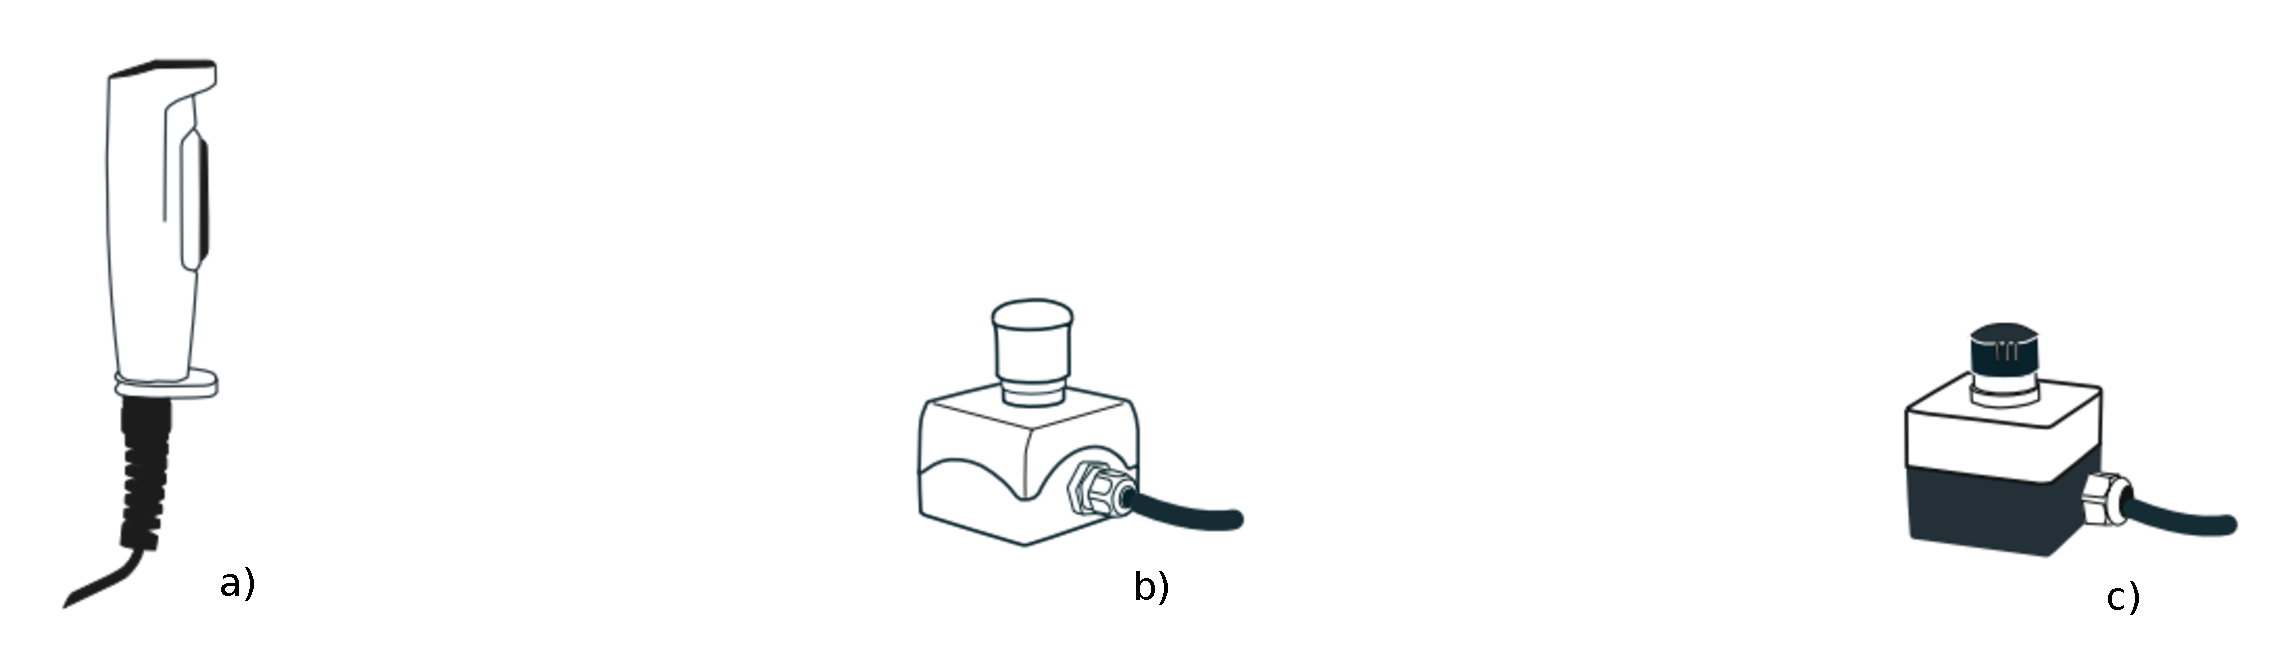
\includegraphics[width=\textwidth]{panda_safety_devices}
	\caption{Panda safety devices. (a) External enabling device; (b) External activation device; (c) Emergency stop device. Courtesy of Franka Emika GmbH and adapted from Panda user handbook of 2018.}
	\label{fig:panda_safety_devices}
\end{figure}

% subsection robotic_system_physical_description_safety_devices

\subsection*{Host PC}
\label{subsec:robotic_system_physical_description_hostpc}

The Host PC is the computer that the robot operator uses to access the Desk interface and run the custom controllers code. This computer should be connected directly to Control if using \gls{fci}, otherwise it can be connected directly to the Panda Arm. To use Desk, the computer only needs an ethernet port and a web browser. To use \gls{fci}, the computer also needs to be running a real time operating system kernel, and have the CPU in performance mode. The preparation of the Host PC to operate under \gls{fci} will be described on the section \ref{sec:robotic_system_integration_ros}.

% subsection robotic_system_physical_description_hostpc

% section robotic_system_physical_description

% ====================================
% = Robot Constraints and Kinematics =
% ====================================

\section{Robot Constraints and Kinematics}
\label{sec:robotic_system_constraints_kinematics}

To fully analyse and be able to model the Panda robotic arm on another system the robot constraints and kinematics must be known. Both the constraints and kinematics are vital for the implementation of the control architecture.

\subsection{Kinematic Chain}
\label{robotic_system_constraints_kinematics_kinematic_chain}

As previously stated, Panda is a robotic arm with seven degrees of freedom. It can be considered a 7R or RRRRRRR type robot, because all its joints are revolute. The model representation using conventional symbols is shown on Figure \ref{fig:panda_joint_model_representation}.\\

\begin{figure}[htbp]
    \centering
	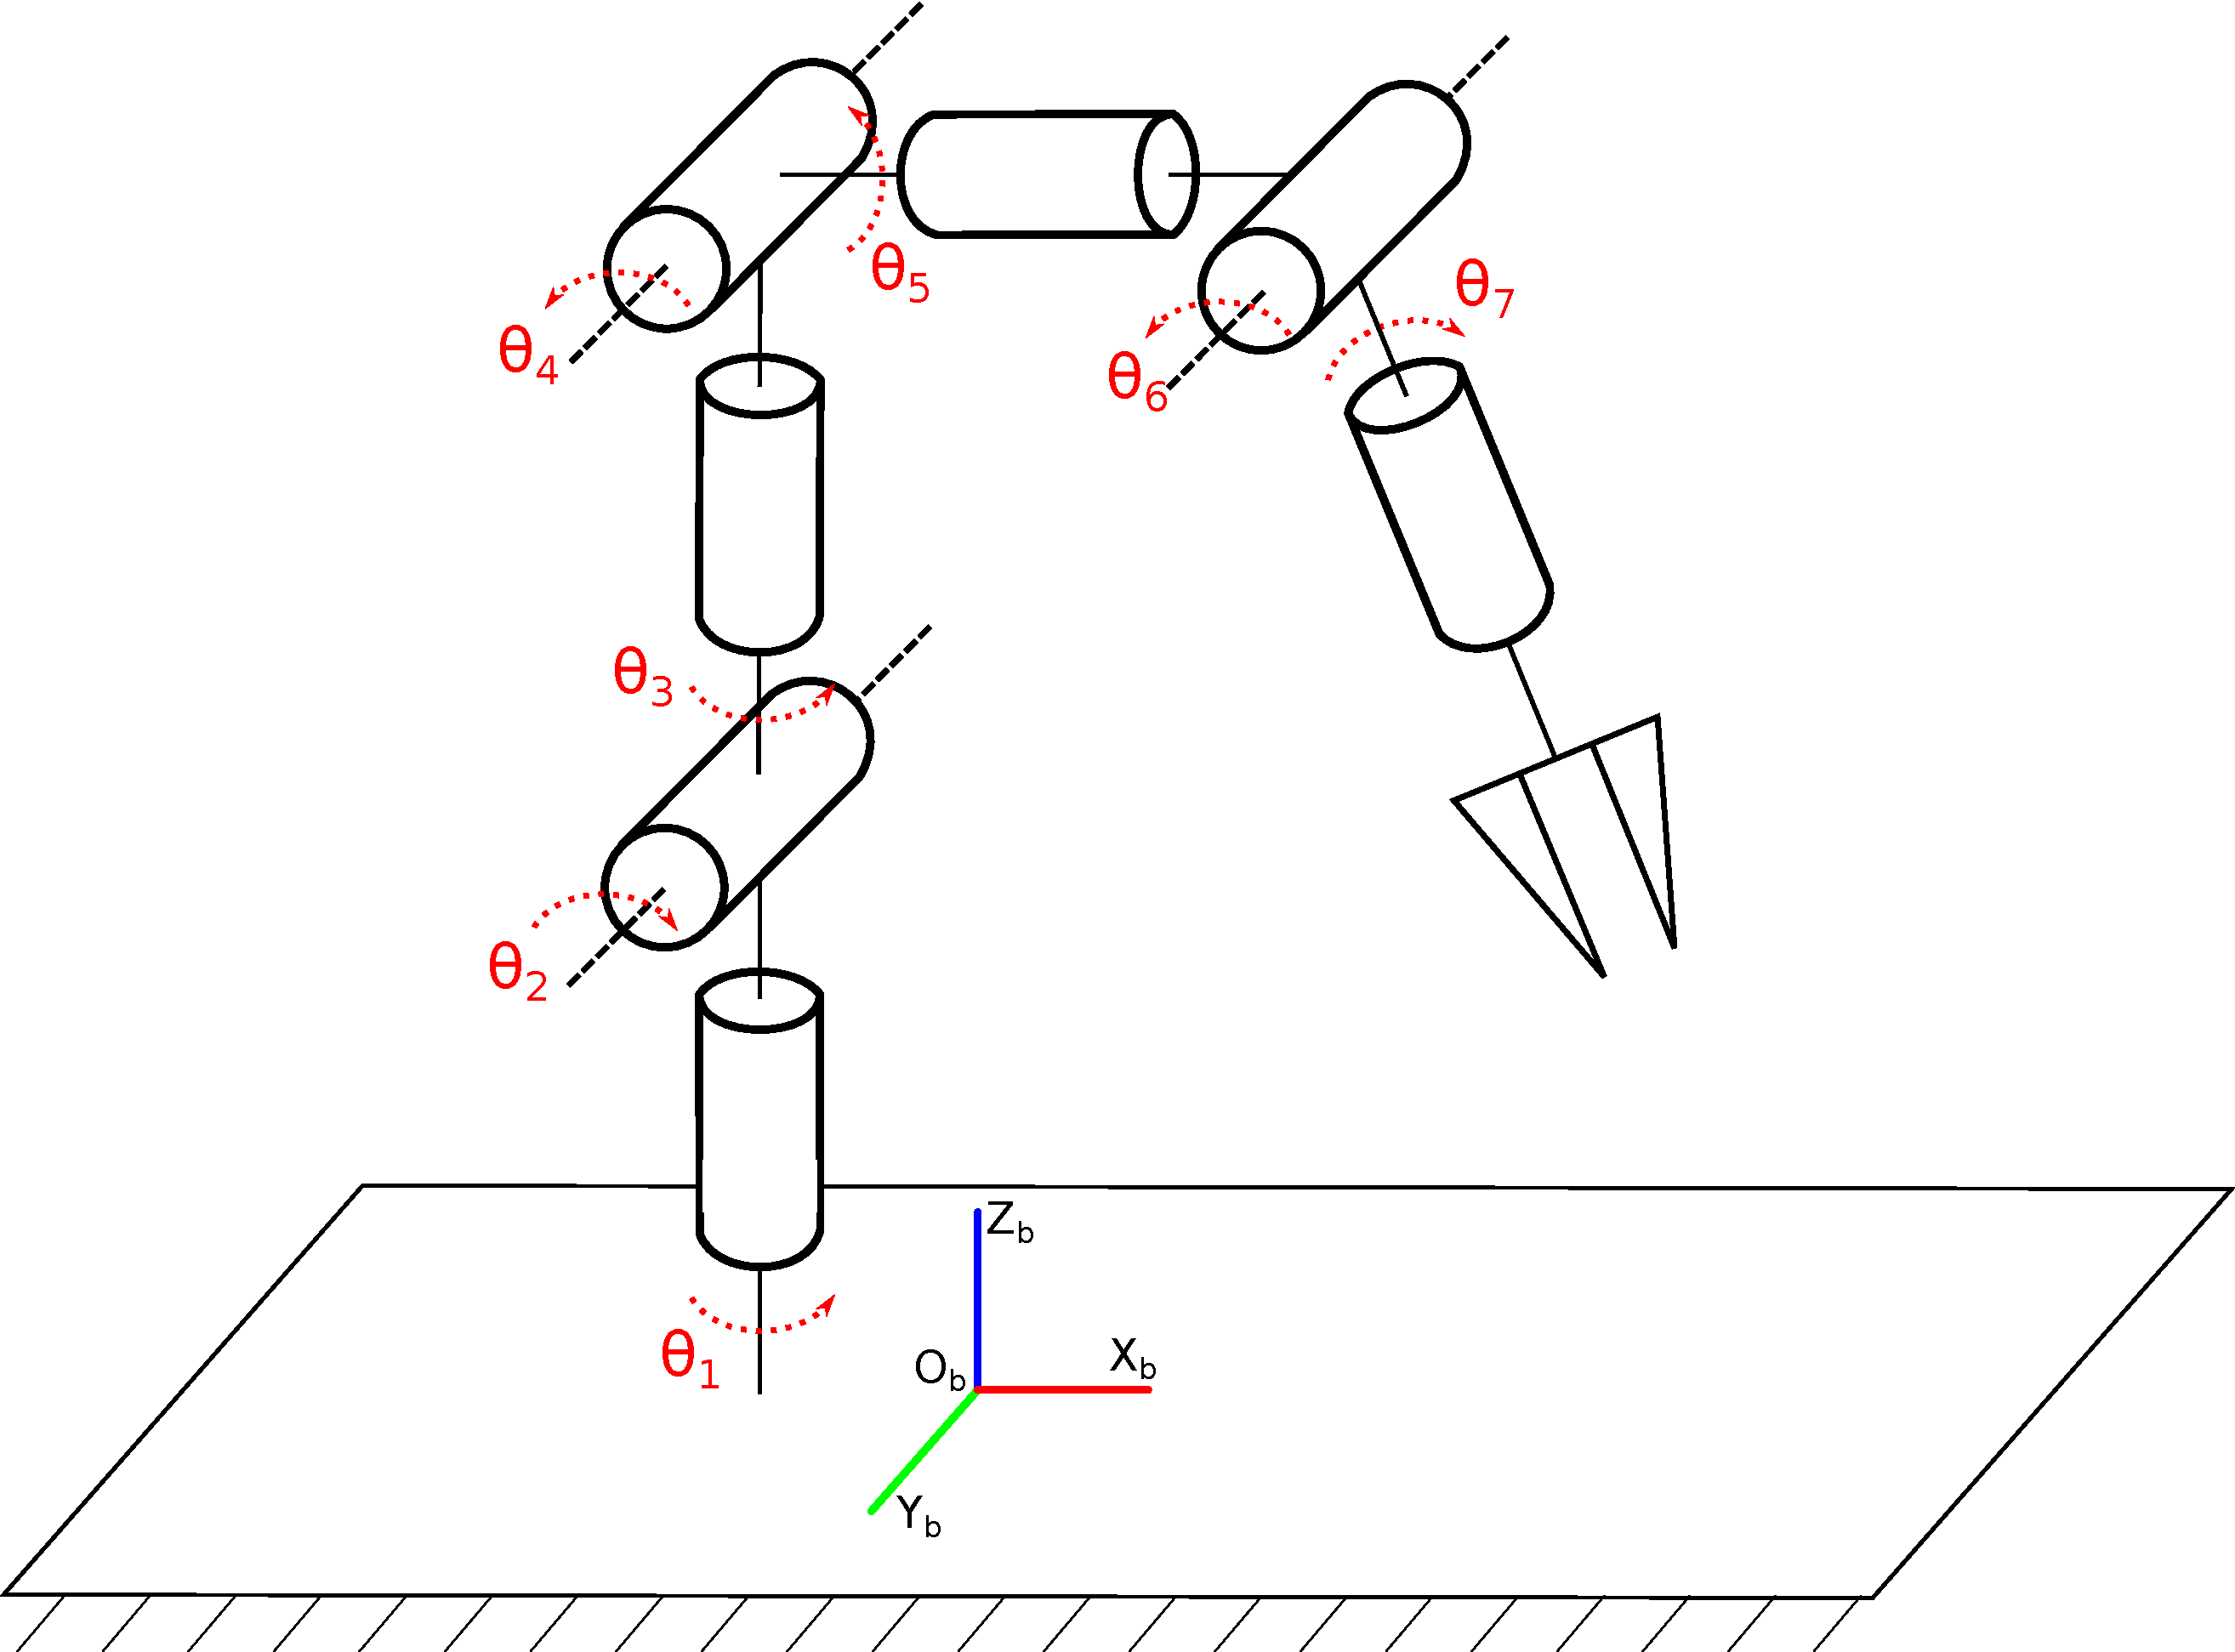
\includegraphics[width=.55\textwidth]{panda_joint_model_representation}
	\caption{Panda robotic arm model representation.}
	\label{fig:panda_joint_model_representation}
\end{figure}

The \glsfirst{fk} chain can be defined by the \glsfirst{dh} parameters. Figure \ref{fig:panda_fci_dh_parameters} presents the reference frames locations used to obtain the \gls{dh} parameters listed on table \ref{tab:panda_dh_parameters}.

\begin{table}[htbp]
    \caption{Panda's \gls{dh} parameters. Courtesy of Franka Emika GmbH from \cite{FrankaEmikaGmbH_fci_documentation}.}
    \centering
    \begin{tabular}{c|c|c|c|c}
        \toprule
        \textbf{Joint} & \textbf{$a$ (m)} & \textbf{$d$ (m)} & \textbf{$\alpha$ (rad)} & \textbf{$\theta$ (rad)} \\
        \midrule
         Joint 1 & 0 & 0.3330 & 0 & $\theta_1$ \\
         \midrule
         Joint 2 & 0 & 0 & $-\frac{\pi}{2}$ & $\theta_2$ \\
         \midrule
         Joint 3 & 0 & 0.3160 & $\frac{\pi}{2}$ & $\theta_3$ \\
         \midrule
         Joint 4 & 0.0825 & 0 & $\frac{\pi}{2}$ & $\theta_4$ \\
         \midrule
         Joint 5 & -0.0825 & 0.3840 & $-\frac{\pi}{2}$ & $\theta_5$ \\
         \midrule
         Joint 6 & 0 & 0 & $\frac{\pi}{2}$ & $\theta_6$ \\
         \midrule
         Joint 7 & 0.0880 & 0 & $\frac{\pi}{2}$ & $\theta_7$ \\
         \midrule
         Flange & 0 & 0.1070 & 0 & 0 \\
         \bottomrule
    \end{tabular}
    \label{tab:panda_dh_parameters}
\end{table}


\begin{figure}[htbp]
    \centering
	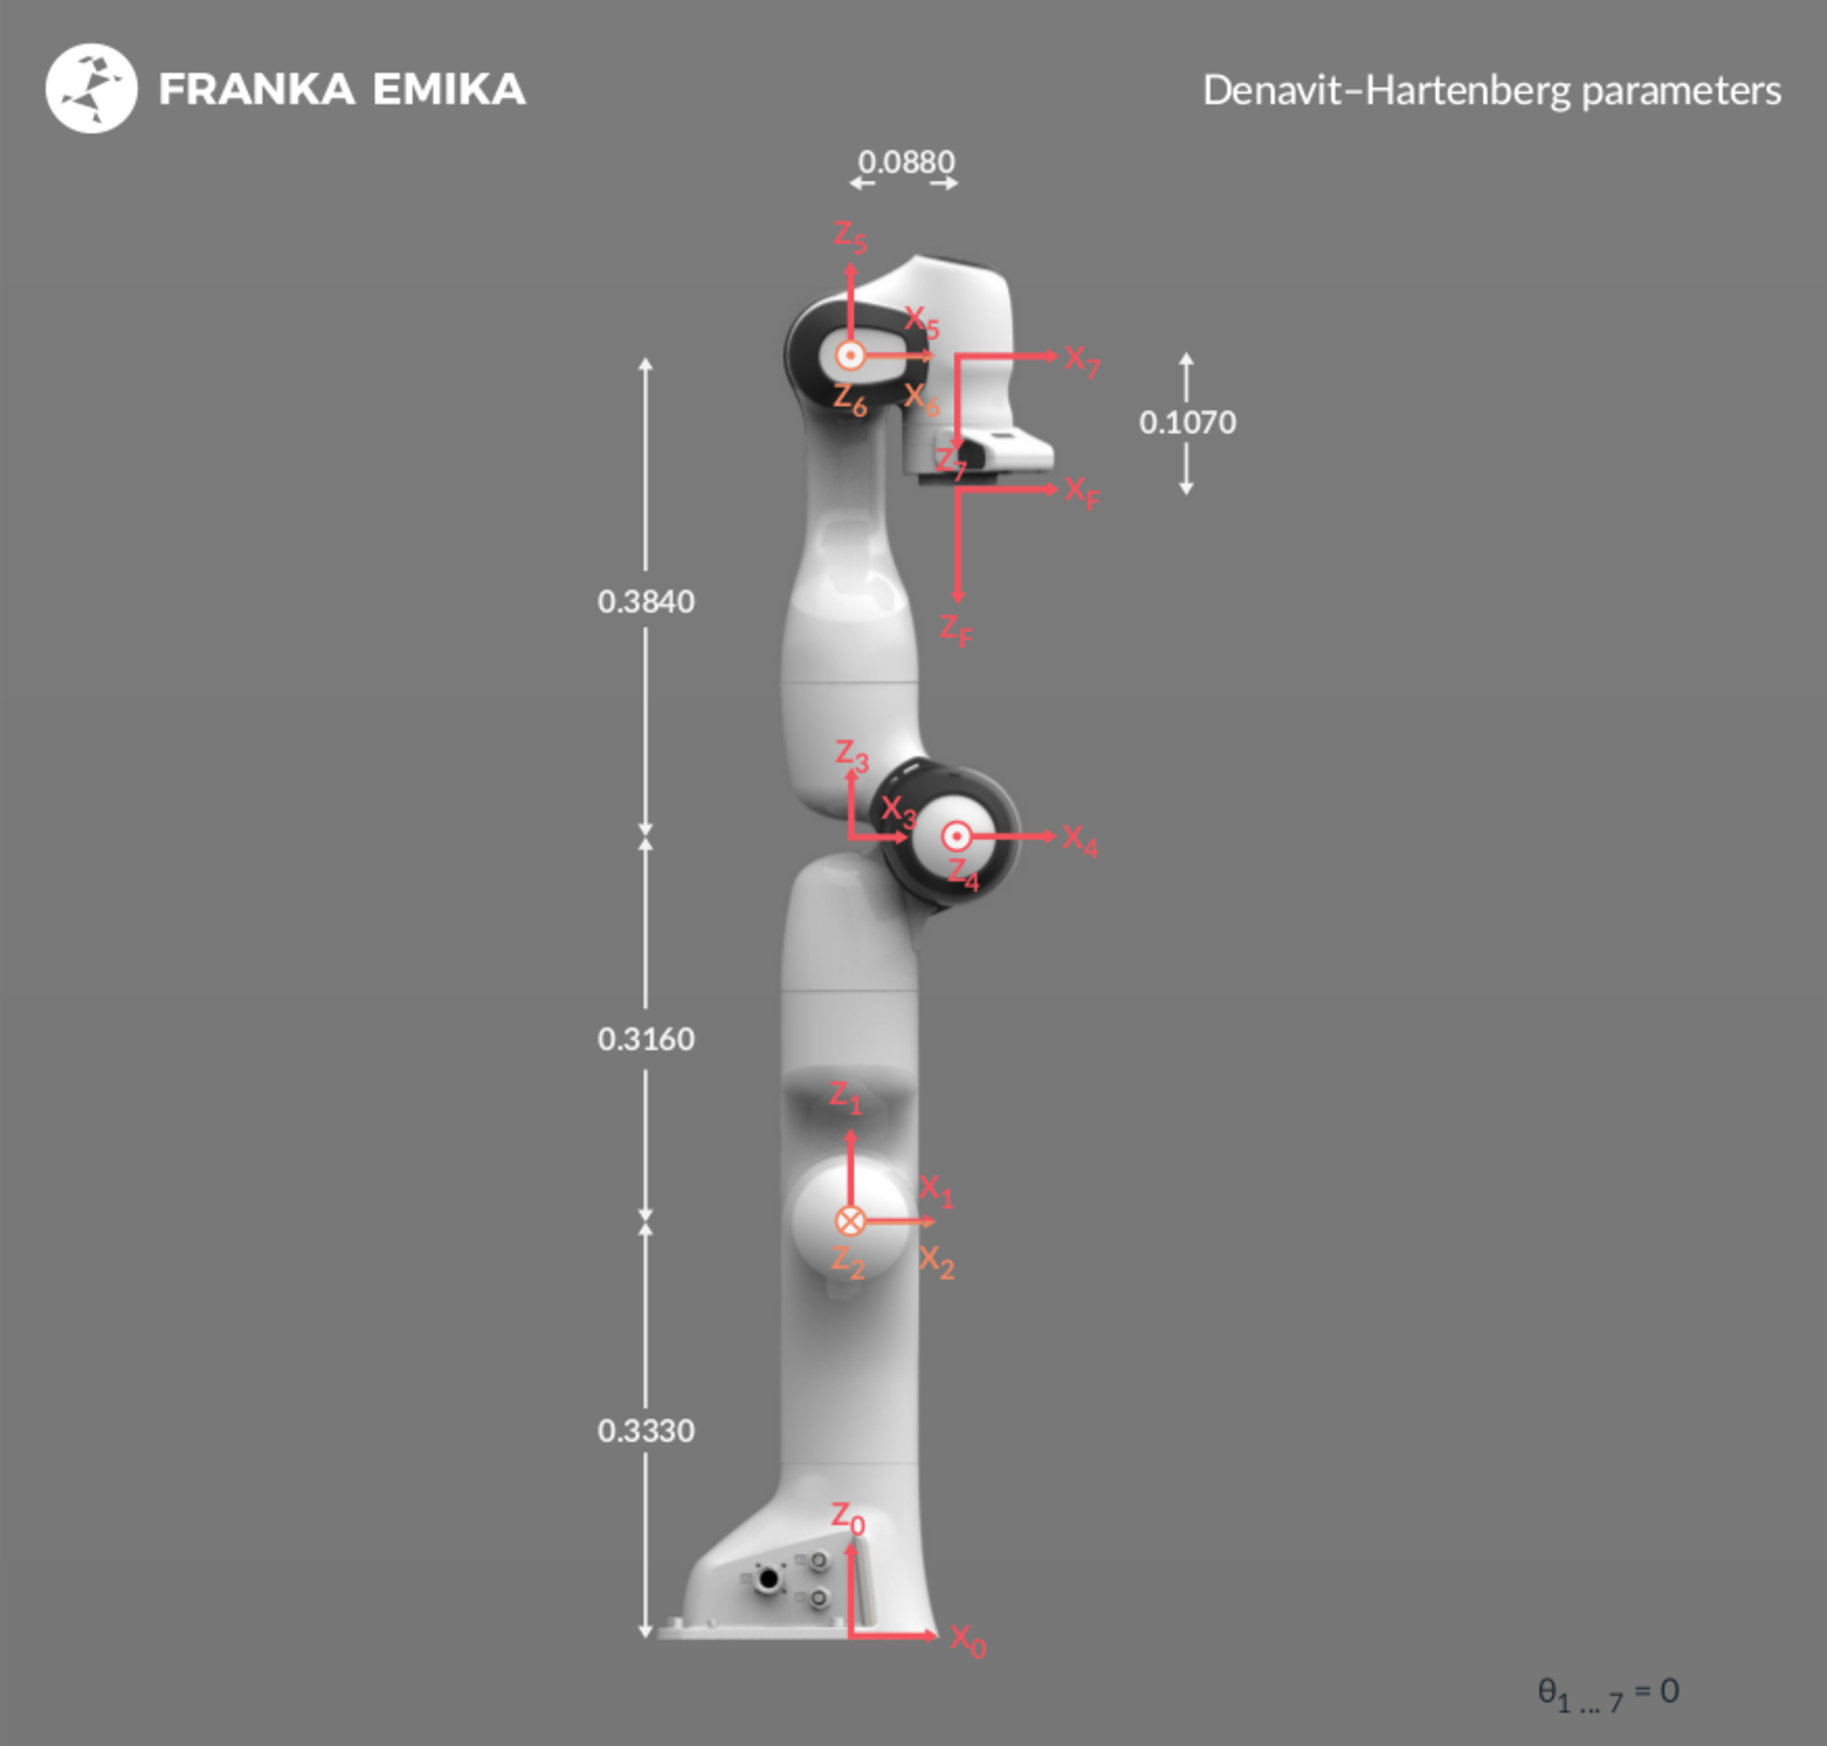
\includegraphics[width=.8\textwidth]{panda_fci_dh_parameters}
	\caption{Panda's kinematic chain. Courtesy of Franka Emika GmbH and adapted from \cite{FrankaEmikaGmbH_fci_documentation}.}
	\label{fig:panda_fci_dh_parameters}
\end{figure}

% subsection robotic_system_constraints_kinematics_kinematic_chain

\subsection{Joint \& Cartesian Limits}
\label{robotic_system_constraints_kinematics_joint_cartesian_limits}

All Panda's joint have physical limits that must be respected to conserve the robot integrity. These limits are both mechanical and kinematic. They are listed on table \ref{tab:panda_joint_limits}.

Besides joint limits, movement in Cartesian space also has its limits. Table \ref{tab:panda_cartesian_limits} presents such limits for speed, acceleration and jerk, for rotation, translation and elbow movement.

\begin{table}[htbp]
    \caption{Panda's joints physical and kinematic limits. Courtesy of Franka Emika GmbH from \cite{FrankaEmikaGmbH_fci_documentation}.}
    \centering
    \begin{tabular}{c|c|c|c|c|c|c|c|c}
        \toprule
        \textbf{Name} & \textbf{Joint 1} & \textbf{Joint 2} & \textbf{Joint 3} & \textbf{Joint 4} & \textbf{Joint 5} & \textbf{Joint 6} & \textbf{Joint 7} & \textbf{Unit} \\
        \midrule
        $\boldsymbol{q}_{max}$ & 2.8973 & 1.7628 & 2.8973  & -0.0698 & 2.8973 & 3.7525 & 2.8973 & \si{\radian}\\
        $\boldsymbol{q}_{min}$ & -2.8973 & -1.7628 & -2.8973 & -3.0718 & -2.8973 & -0.0175 & -2.8973 & \si{\radian} \\
        $\dot{\boldsymbol{q}}_{max}$ & 2.1750 & 2.1750 & 2.1750 & 2.1750 & 2.6100 & 2.6100 & 2.6100 & \si{\radian\per\second} \\
        $\ddot{\boldsymbol{q}}_{max}$ & 15 & 7.5 & 10 & 12.5 & 15 & 20 & 20 & \si{\radian\per\second\squared} \\
        $\dddot{\boldsymbol{q}}_{max}$ & 7500 &	3750 &	5000 & 6250 & 7500 & 10000 & 10000 & \si{\radian\per\second\cubed} \\
        $\boldsymbol{\tau}_{jmax}$ & 87 & 87 & 87 & 87 & 12  & 12 & 12 & \si{\newton\meter} \\
        $\dot{\boldsymbol{\tau}}_{jmax}$ & 1000 & 1000 & 1000 & 1000 & 1000 & 1000 & 1000 & \si{\newton\meter\per\second} \\
        \bottomrule
    \end{tabular}
    \label{tab:panda_joint_limits}
\end{table}

\begin{table}[htbp]
    \caption{Panda's Cartesian limits, speed, acceleration and jerk. Courtesy of Franka Emika GmbH from \cite{FrankaEmikaGmbH_fci_documentation}.}
    \centering
    \begin{tabular}{c|c|c|c}
        \toprule
        \textbf{Name} & \textbf{Translation} & \textbf{Rotation} & \textbf{Elbow} \\
        \midrule
        $\dot{\boldsymbol{p}}_{max}$ & 1.7000 \si{\meter\per\second} & 2.5000 \si{\radian\per\second} & 2.1750 \si{\radian\per\second} \\
        $\ddot{\boldsymbol{p}}_{max}$ & 13.0000 \si{\meter\per\second\squared} & 25.0000 \si{\radian\per\second\squared} & 10.0000 \si{\radian\per\second\squared} \\
        $\dddot{\boldsymbol{p}}_{max}$ & 6500.0000 \si{\meter\per\second\cubed} & 12500.0000 \si{\radian\per\second\cubed} & 5000.0000 \si{\radian\per\second\cubed} \\
        \bottomrule
    \end{tabular}
    \label{tab:panda_cartesian_limits}
\end{table}

% subsection robotic_system_constraints_kinematics_joint_cartesian_limits

% section robotic_system_constraints_kinematics

% ==========================
% = Operation =
% ==========================

\section{Operation}
\label{sec:robotic_system_operation}

The Panda robotic arm can be operated in two modes. The operator can use the Desk interface or custom controllers using \gls{fci}. But before describing the way to operate the robot, its installation and security aspects will be addressed first.

\subsection{Installation}
\label{subsec:robotic_system_operation_installation}

In order to guarantee proper operation the robotic arm must be installed according to specifications provided on the user manual.\\

The site of installation must be: indoors; not exposed to direct sunlight; have no vibrations; and no magnetic fields. The last two are very important. 

The sensitivity of the mechatronic systems demand a very stable platform to install the robotic arm. Installing it on a fragile platform can limit the robot operation or jeopardize the safety of the operator. According to the user manual the following maximum forces must be supported during static and dynamic operation (Fig. \ref{fig:panda_installation_forces}):

\begin{itemize}
    \item vertical force: 410 N
    \item horizontally force: 300 N
    \item tilting torque: 280 Nm
    \item torque around axis 1: 90 Nm
\end{itemize}

\begin{figure}[htbp]
    \centering
	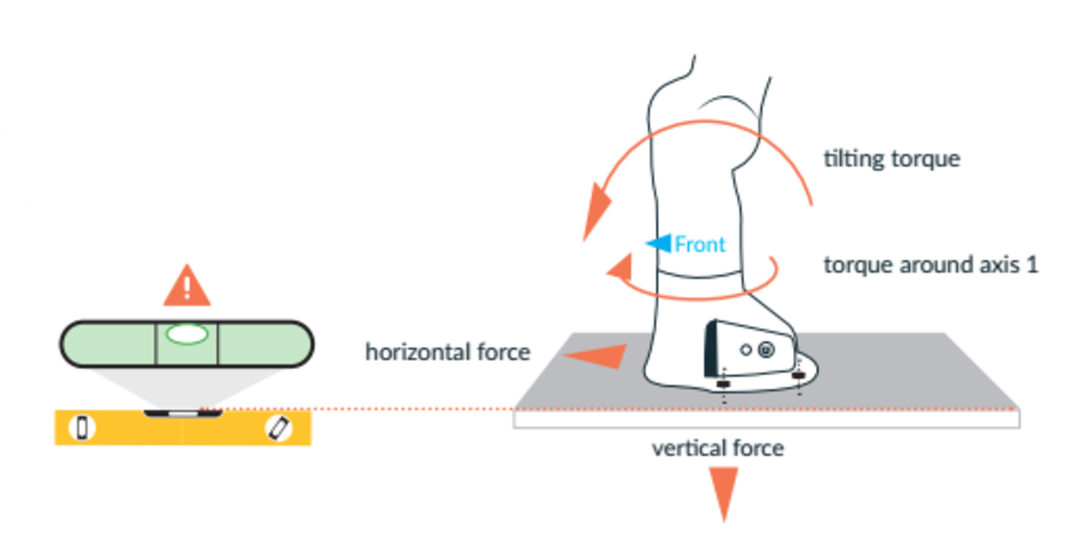
\includegraphics[width=.8\textwidth]{panda_installation_forces}
	\caption{Installation considerations for Panda robotic arm. Courtesy of Franka Emika GmbH and adapted from Panda user handbook of 2018.}
	\label{fig:panda_installation_forces}
\end{figure}

The demand for a stable platform to install the robot may also limit its mobility. A mobile platform may not be cable of supporting the forces mentioned on the previous paragraph for static and dynamic operation.

The limitation of no magnetic fields on the installation site means that the robotic arm cannot be used in conjunction with MRI machines and other magnetically active devices.\\

For more details on how to effectively mount the robotic arm, control, hand, and do all the connections, read the user manual which comes in the system's package.

% subsection robotic_system_operation_installation

\subsection{Safety}
\label{subsec:robotic_system_operation_safety}

Like with any robotic system, it is very important to take into consideration the system's and operator's safety. Even more when considering autonomous operation. A few aspects regarding Panda's safety will be mentioned. More in depth details are available on the user manual.

\subsubsection*{Possible Dangers}
\label{subsubsec:robotic_system_operation_safety_possible_dangers}

According to the user manual, the list of possible dangers associated with the operation of Panda robotic arm are the following:

\begin{itemize}
    \item Mechanical dangers
    \begin{itemize}
        \item Crushing
        \item Shearing
        \item Impact, puncture, penetration
    \end{itemize}
    \item Electrical hazards
    \begin{itemize}
        \item Electric shock when touching live part
    \end{itemize}
    \item Environmental hazards
    \begin{itemize}
        \item Crushing, shearing, impact, puncture, penetration
    \end{itemize}
    \item Combined hazards
    \begin{itemize}
        \item Crushing, shearing, impact, puncture, penetration
    \end{itemize}
\end{itemize}

% subsubsection robotic_system_operation_safety_possible_dangers

\subsubsection*{Hazardous, Safe and Collaborative Areas}
\label{subsubsec:robotic_system_operation_safety_hazardous_safe_collaborative_areas}

Three important concepts regarding safety are presented on the user manual. These are \textbf{Hazardous Area}, \textbf{Safe Area} and \textbf{Collaborative Area}.\\

The Hazardous Area is the operating area in which the arm executes its tasks. It corresponds to a circular area limited by the arm's reach (Fig. \ref{fig:panda_hazardous_safe_collaborative_areas}).

The Safe Area is an area where humans are separated from the hazardous area by constructive or protective measures. In general, during normal operation, being outside of the operating area will not present a safety risk (Fig. \ref{fig:panda_hazardous_safe_collaborative_areas}).

Collaborative Area corresponds to the operating space when it is used by humans and the robot. The area is shared by both, but not used at the same time. Because the shared is not constant, normally only a small part of the operating space is used collaboratively, allowing for better safety control \ref{fig:panda_hazardous_safe_collaborative_areas}).\\

In our particular application, the patient will always be inside the hazardous area. This demands a higher consideration for the safety measures. The operator may be inside the hazardous area when manipulating the robotic arm.

\begin{figure}[htbp]
    \centering
	\raisebox{-0.5\height}{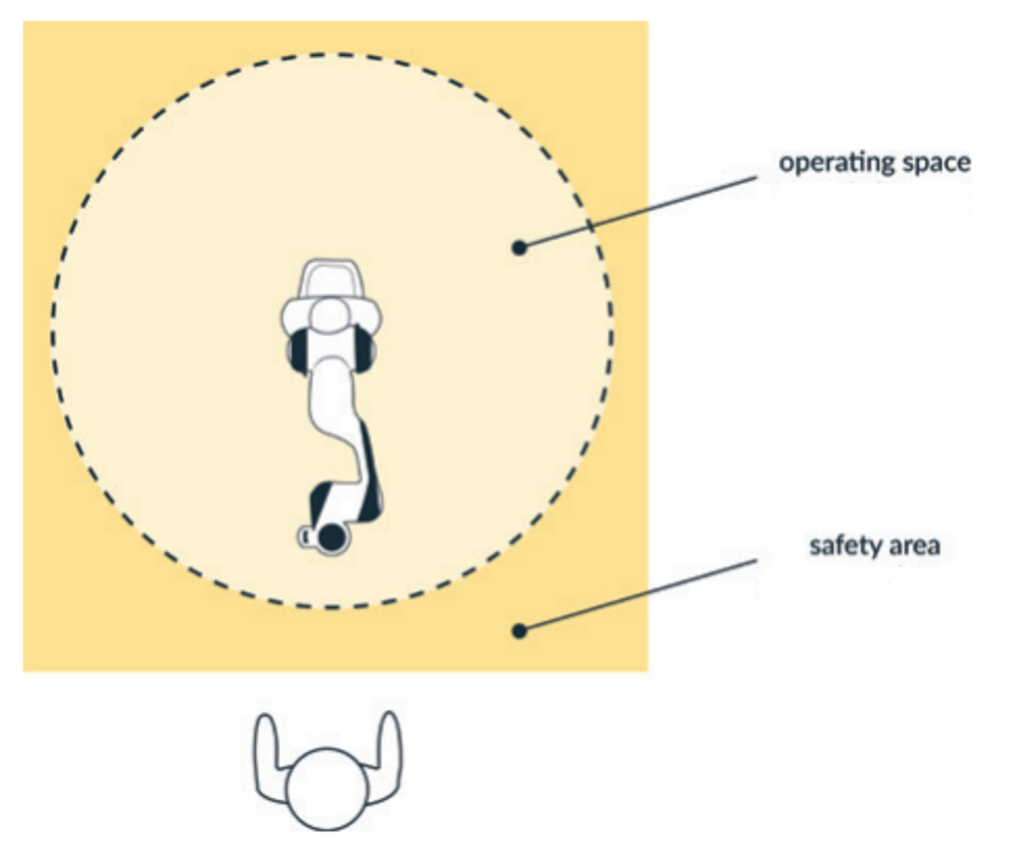
\includegraphics[width=.5\textwidth]{panda_hazardous_safe_areas}}
	\hspace{0.1in}
	\raisebox{-0.35\height}{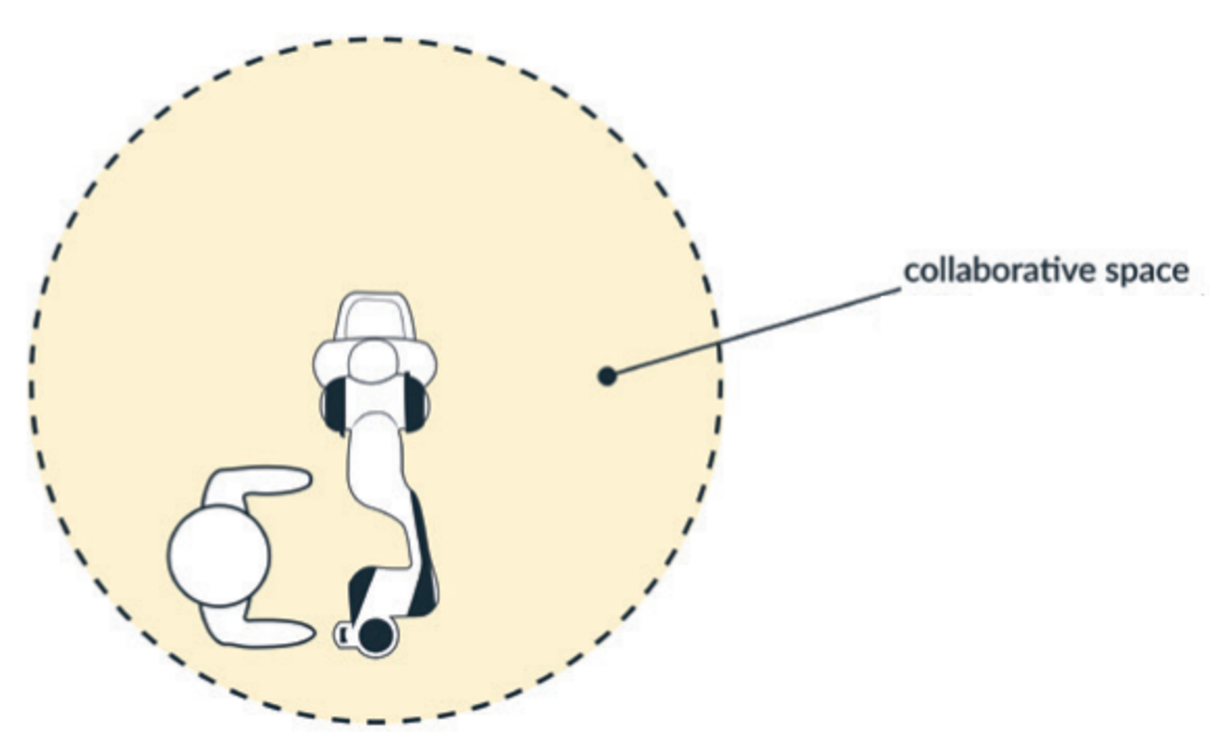
\includegraphics[width=.45\textwidth]{panda_collaborative_space}}
	\caption{Panda Hazardous, Safe and Collaborative Areas. Courtesy of Franka Emika GmbH and adapted from Panda user handbook of 2018.}
	\label{fig:panda_hazardous_safe_collaborative_areas}
\end{figure}

% subsubsection robotic_system_operation_safety_hazardous_safe_collaborative_areas

\subsubsection*{Stopping Mechanisms}
\label{subsubsec:robotic_system_operation_safety_stopping_mechanisms}

Panda comes with three safety stop mechanisms: the external enabling device; external activation device; and emergency stop device. These were previously described on section \ref{sec:robotic_system_physical_description} and shown on Figure \ref{fig:panda_safety_devices}.

The emergency stop device cuts power from the robotic arm and control. It is the best safety mechanism to completely deactivate the system. The other two mechanisms provide some safety control during robot operation. They should always be used and be in proximity of the operator to be accessed immediately if needed.

% subsubsection robotic_system_operation_safety_stopping_mechanisms

\subsubsection*{Fail Safe Locking System}
\label{subsubsec:robotic_system_operation_safety_fail_safe_locking_system}

The last important safety mechanism to mention is the fail safe locking system. This mechanism is installed on each joint and guarantees that the robotic arm keeps its pose when the power supply is disconnected. It is important to mention that the locking system still allows a certain degree of movement before the lock. It is more evident on joints that move with gravity. This must be considered during manipulation.

% subsubsection robotic_system_operation_safety_fail_safe_locking_system

\subsubsection*{Status Indicators}
\label{subsec:robotic_system_operation_safety_status_indicators}

During operation it is important to have feedback on the system status. Panda comes with two LED status indicators, one on the robot base and the other on the Pilot.

The different status are distinguished by their color and activity. Figure \ref{fig:panda_status_indicators} shows the relation between the LED colors and robot state.

\begin{figure}[htbp]
    \centering
	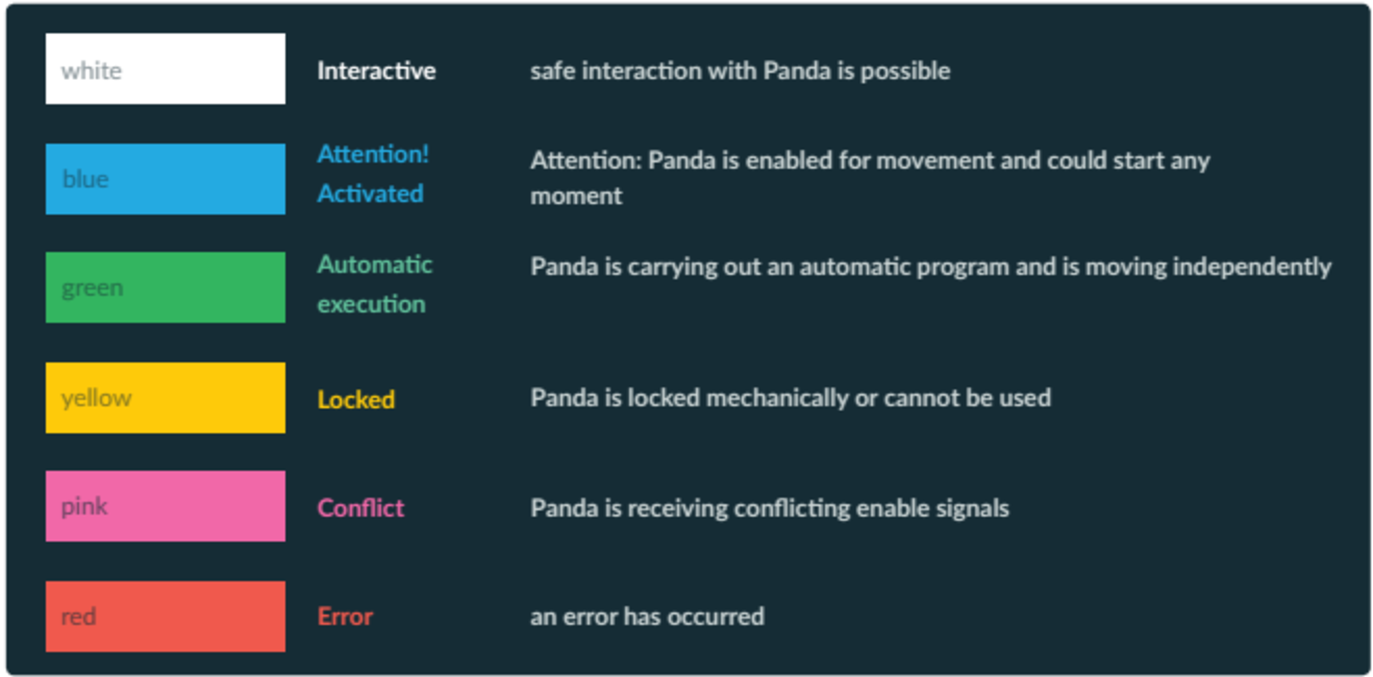
\includegraphics[width=\textwidth]{panda_status_indicators}
	\caption{Panda status indicators color chart. Courtesy of Franka Emika GmbH and adapted from Panda user handbook of 2018.}
	\label{fig:panda_status_indicators}
\end{figure}

% subsubsection robotic_system_operation_safety_status_indicators

% subsection robotic_system_operation_safety

\subsection{Operation with Desk}
\label{subsec:robotic_system_operation_desk}

Desk is a web application that allows the operator to control the robot arm without any programming. The user can create various Tasks. Each task is an independent set of movements the robot should execute. Each task is composed by different configurable apps. Some correspond to movements, others to general task configuration. Figure \ref{fig:panda_desk_interface} presents an overview of Desk user interface.

\begin{figure}[htbp]
    \centering
	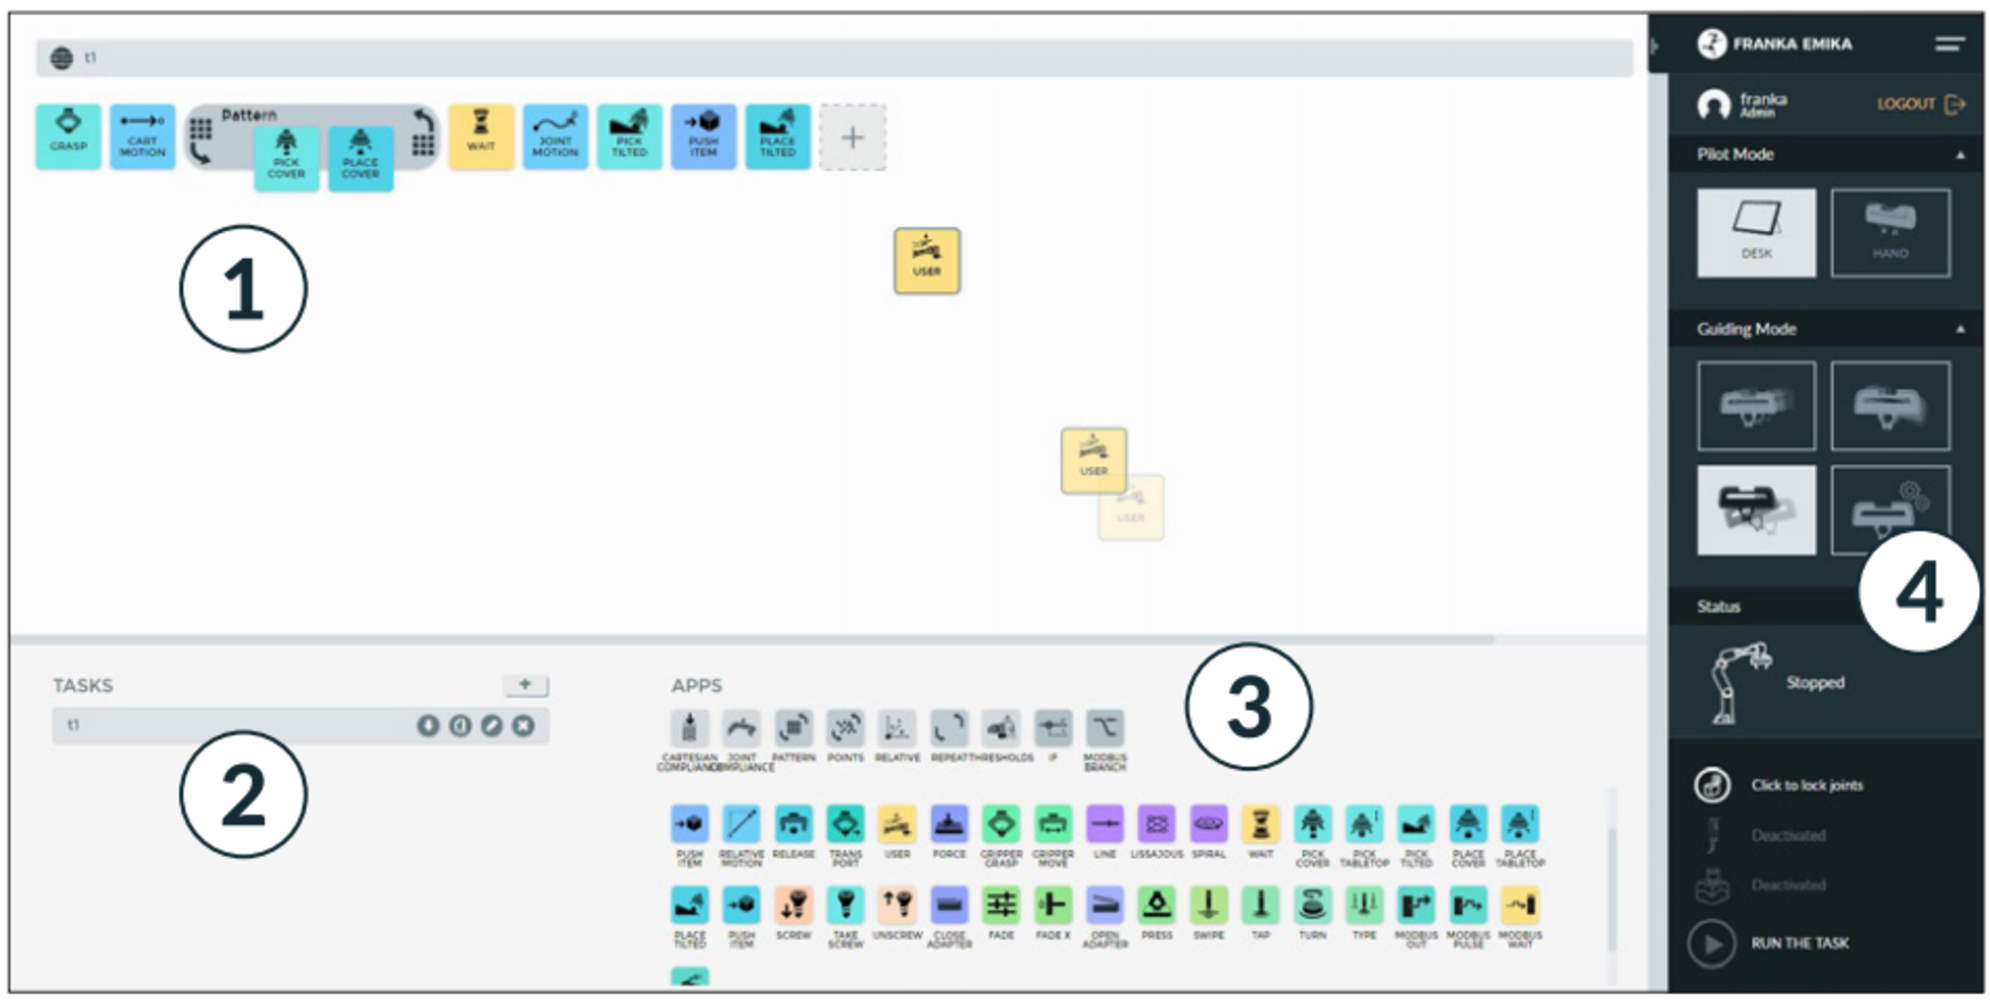
\includegraphics[width=\textwidth]{panda_desk_interface}
	\caption{Desk user interface. (1) Timeline area where apps are lined up to build up the task. (2) Task area. (3) App Area. The list of available apps are displayed here and can be placed on the timeline via Drag-and-Drop. (4) Side Bar. It is possible to select the pilot and guiding modes. It also shows the robot status and task execution control. Courtesy of Franka Emika GmbH and adapted from Panda user handbook of 2018.}
	\label{fig:panda_desk_interface}
\end{figure}

Because Desk was not used during these thesis the complete operation procedure will not be explained. For more details, refer to the user manual.

% subsection robotic_system_operation_desk


\subsection{Startup Procedure}
\label{subsec:robotic_system_operation_startup}

Even when controlling the robot through \gls{fci}, Desk should always be the first interface to use when the robot is connected. This is so because after powering Control the fail safe locks are activated and Desk is needed to deactivate. The startup procedure should be:

\begin{enumerate}
    \item Verify that the external activation device is locked.
    \item Power on Control.
    \item Open a web browser and visit \url{https://<fci-ip>/} if Host PC is connected to Control or \url{https://robot.franka.de/} if connected directly to the robotic arm. Wait for initialisation end. The status light should be blinking yellow.
    \item After initialisation is done (status light yellow), on Desk's interface Side Bar, click the \textbf{Unlock Joints} button to disable fail safe locking system. The robot moves during unlocking. When it is done the status light turns white.
    \item Unlock the external activation device. The status light turns blue.
    \item The robot is ready to be operated via Desk or \gls{fci}.
\end{enumerate}

% subsection robotic_system_operation_startup

% section robotic_system_operation

% ==========================
% = Integration with ROS =
% ==========================

\section{Integration with \gls{ros}}
\label{sec:robotic_system_integration_ros}

To control Panda robotic arm, the \gls{fci} was used. Franka control interface allows direct control of the panda joints via custom control architectures. \gls{fci} can be accessed via two open source components: a C++ library, \textit{libfranka}; and a \gls{ros} integration, \textit{franka\_ros}, made of a set of packages that include support for ROS Control, MoveIt! and robot models for RViz and simulation on Gazebo. The integration details are described on appendix \ref{app:ros_setup}.

% section robotic_system_integration_ros

% ==========================
% = Integration with Gazebo =
% ==========================

\section{Integration with Gazebo}
\label{sec:robotic_system_integration_gazebo}

Gazebo is robotics simulator commonly used with \gls{ros} to create various types of simulation environments. By using a simulator, various algorithms can be tested on a sandbox environment before testing with the real systems. This helps the development process and reduces the potential for hardware faults related to programming errors.\\

For this thesis, Gazebo was important to simulate the robotic arm and the depth camera. The whole system was tested on a simulated environment and also with real hardware. The integration details are described on appendix \ref{app:gazebo_setup}.

% section robotic_system_integration_gazebo